\documentclass[10pt]{unlsilabsop}
\title{Destructive wirebond acceptance test of HDI}
\date{August 6, 2015}
\author{Frank Meier Aeschbacher}
\approved{Frank Meier Aeschbacher}
\sopid{209}
\sopversion{v1}
\sopabstract{Describes the procedure to test HDI for suitability to wirebonding. This destructive test is optional and makes HDI not suitable for manufacturing without reworking.}
\begin{document}

\maketitle

%------------------------------------------------------------------
\section{Scope}
This test is mainly for type testing of samples from HDI batches. The test uses ROC wirebond pads to gain large statistics.

HDI can be reworked by removing all traces of wirebonds. Such HDI can be reused without restriction because the normal location of the bond is in the center of the pad whereas this test places it at the two ends of the pad.

%------------------------------------------------------------------
\section{Purpose}
Bondability is a critical quality criterion for HDI. This test allows to characterize batches of HDI for suitability for wirebonding.

%------------------------------------------------------------------
%\section{Definitions}
%\begin{itemize}
%\item \textbf{bla} Text
%\end{itemize}

%------------------------------------------------------------------
%\section{Responsibilities}

%------------------------------------------------------------------
\section{Equipment}

\begin{itemize}
    \item Wirebonder: Delvotec 56XX
    \item Bond head: Delvotec 5630
    \item Bond wedge: SPT UT45A-W-2030-1.00-C, having a bond flat size of 3\,mils
    \item Pull tester: PH-100
    \item Pull hook: WEP-00001
    \item Chuck
    \item Bond wire: aluminium 25\,$\mu$m diameter, Heraeus ALW-29S on 2" spool
    \item Tweezers for wire handling
    \item Test coupon
    \item In case back side of HDI is too rough to be held by vacuum:
    \begin{itemize}
	\item Double sided adhesive tape, Scotch 3M 238
	\item Kapton tape, 1/4", 1 mil thickness
	\item Kapton tape, 1", 5 mil thickness
	\item Cotton swabs
    \end{itemize}
\end{itemize}

%------------------------------------------------------------------
\subsection{Bonder setting}

Table \ref{tbl:bondpar} lists the bond settings which have to be used by the operator. Different sets of parameters are available and must be specified upon requesting the test.
\begin{description}
    \item[Set A:] Lower end set of parameters. HDI with bonding issues will show up low pull strengths in testing or missing bonds when making them.
    \item[Set B:] Set used for problematic HDI. Such items will show better bondability than with Set A but good HDI will show overwelding (lower pull strengths than with Set A and dominance of heel breaks).
\end{description}
In order to maintain comparability, using settings other than listed in this table are only allowed upon special request and need explicit mentioning in the test report. Table \ref{tbl:otherpar} lists general machine settings to be used.

\begin{table*}[hH]
\begin{center}
\caption{Bond parameter settings for bonds from HDI to ROC and HDI to sensor HV pad. Bond settings are for both bonds (first and second).}
\label{tbl:bondpar}

\bigskip

\begin{tabular}{lc|c|c}
\toprule
Parameter & Unit & Set A & Set B  \\
    \midrule
US Time      &  ms    &  25 &  50 \\
B-Force      &  cN    &  30 &  30 \\
US Power     & digit  & 140 & 155 \\
TD Steps     & $\mu$m &  12 &  15 \\
    \midrule
Z-Presign    & \%     &  65 &  65 \\
Loop Height  & $\mu$m &   0 &   0 \\
LoopH-Fct    & \%     & 125 & 125 \\
ClampFlag    & --     &   0 &   0 \\
XY LoopH-Fct & \%     &  50 &  50 \\
Z-Delay      & \%     &   0 &   0 \\
   \bottomrule
\end{tabular}
\end{center}
\end{table*}

\begin{table*}[hH]
\begin{center}
\caption{Machine parameter settings. Settings marked with an asterisk (*) may vary according to operator's preference.}
\label{tbl:otherpar}

\bigskip

\begin{tabular}{lcc}
\toprule
Parameter          & Unit   & Value \\
\midrule
Workheight 1       & $\mu$m & 24182 *\\
Workheight 2       & $\mu$m & 36293 * \\
\multicolumn{2}{l}{Use Diagonal Tolerance} & yes \\
Diagonal Tolerance & $\mu$m & 100 \\
TD Ramp            & $\mu$m & 300 \\
Clamp value        & digit  & 650 \\
Feed               & steps  & 16 \\
Limiter            & steps  & 16 \\
Wire Diameter      & $\mu$m & 25 \\
Production Mode    & --     & 1 \\
Adjust Mode        & --     & 1 \\
Bond Mode          & --     & 0 \\
Monitoring Mode    & --     & 0 \\
\midrule
Motor Z max        & $\mu$m & 40800 \\
    \bottomrule
\end{tabular}
\end{center}
\end{table*}

%------------------------------------------------------------------
\subsection{Pull tester settings}
Table~\ref{tbl:testpar} lists the settings for the pull tester.

\begin{table*}[hH]
\begin{center}
\caption{Pull tester parameter settings.}
\label{tbl:testpar}

\bigskip

\begin{tabular}{lcc}
\toprule
Parameter          & Unit   & Value \\
\midrule
\multicolumn{2}{l}{Testname}           & HDI acceptance test \\
\multicolumn{2}{l}{Sequenzer Mode}     & Manual\\
Lotsize            & 1      & 25 \\
\multicolumn{2}{l}{Grade List}         & PullGrades\\
\multicolumn{2}{l}{Lot Info}           & HDI RevC\\
\multicolumn{2}{l}{Loopheight measure} & off\\
\multicolumn{2}{l}{Destructive}        & yes\\
\multicolumn{2}{l}{Force Grading}      & Always\\
\multicolumn{2}{l}{Step Back}          & Rotate Hook +\\
Feed In Offset (X/Y) & $\mu$m & 200\\
Adjust Offset Z      & $\mu$m & 400 \\
Fallback to          & \%     & 30 \\
Lower Spec Limit     & cN     & 10.0 \\
Test Speed           & $\mu$m/s & 2000 \\
Test Load            & cN     & 20 \\
    \bottomrule
\end{tabular}
\end{center}
\end{table*}

%------------------------------------------------------------------
\section{Procedures}
The test consists of two steps: making bonds and pulling them. If more than one sample needs to be tested at once, it is acceptable to first do the wirebonds on all samples and then configure the machine for pull testing.
\subsection{Step 1: Making bonds}
\begin{enumerate}
    \item Handle bare modules only with proper protection: ESD wristband, gloves, face mask. If HDI are unstuffed, ESD wristband may be omitted.
    \item Configure the bonder for aluminium wedge bonding. Mount the bond head following the manual.
    \begin{enumerate}
	\item Check if bond wire feeds. If in doubt, re-feed wire according to manual.
	\item If bonding for the first time this day: Make a manual test bond on a coupon. Add this to your report.
	\item Check if vacuum is present by reading the gauge. If not, perform the following checks: vacuum pump is on (outside cleanroom), valve is open.
    \end{enumerate}
    \item Depending on how the back side of the HDI has been treated, proceed either way:
    \begin{enumerate}
	\item Place HDI on chuck and turn on vacuum. HDI should be held firmly and no gaps are visible between ROC bond pads and chuck. Chuck should be held firmly, no air sounds and vacuum pressure stays low on the gauge. If not, use one of the following alternative approach:
	\item (Easier to remove HDI afterwards) Place double sided adhesive tape over the holes of the chuck and place HDI on it. Press firmly using a cotton swab along the edges. Make sure no other features (wirebonds, surface mounted parts, etc.) present are damaged.
	\item (For bad cases, Kapton tape will be harder to remove from HDI) Take 5\,mil thick Kapton tape on chuck, sticky side up. Engage vacuum. Place HDI on sticky surface and press down firmly using a cotton swab. HDI should be held down evenly, vacuum pressure should stay low on gauge.
    \end{enumerate}
    If HDI was delivered glued to a glass slide, mock sensor or any other stiff substrate, place on chuck and proceed.
    \item Identify the HDI and record this information.
    \item Load the bond program named \texttt{SOP-209-DestructiveHDItesting-SetX.db}, where \texttt{X} identifies the parameter set.
    \item Check the settings with the test requirements. For the bond parameters, select all wires and check the parameters for first bond, loop, and second bond.
    \item Determine and record the height of the HDI bond pads. Do this in ``Learn chip'', click on $z$ height, move the bond head to a suitable and representative position and hit ``Store trace''. If testing more HDI of the same kind, this step may be omitted for later HDI in the same go.
    \item Run alignment step. Choose one ROC pad and record the number.
    \item Run program. Supervise progress and stop in need, especially when HDI are at risk or wirebonds are continuously missing. No stop needed for an occasional miss. Record number of misses per pad group for one ROC.
    \item At the end of the full cycle, check visually if all wirebonds are present. Do not rebond any missing bonds (it is a test procedure, not for manufacturing).
\end{enumerate}
\subsection{Step 2: Pull testing of bonds}
\begin{enumerate}
    \item Configure the machine for pull testing.
    \item Check vacuum.
    \item Adjust z-height of the pull hook and set lowest level to a safe height.
    \item Adjust microscope to have the hook and the bond under test in focus.
    \item Make destructive pull tests using testname \texttt{HDI acceptance test}. Make $N=25$ pull tests per ROC pad. The remaining bonds are spares to compensate for missed bonds.
    \item Observe every pull through the microscope and rate the failures according to the scheme given in Fig.~\ref{fig:grading}.
    \item Report the results.
\end{enumerate}

\begin{figure}[h]
    \begin{center}
        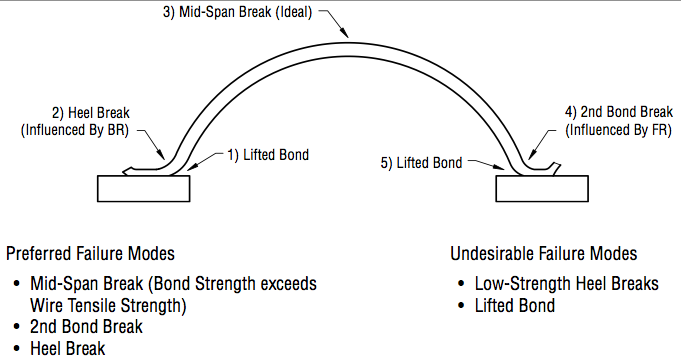
\includegraphics[width=12cm]{img/GradingWedgeBondBreaks.png}
        \caption{Grading of wedge bond breaks. The number signifies the code to be used. Image source: CoorsTek}
        \label{fig:grading}
    \end{center}
\end{figure}

%------------------------------------------------------------------
\section{Documentation}
The following information needs to be recorded in the report for the UNL logbook using the templated provided on the TWiki:
\begin{itemize}
\item Date, time (start--end) and operator name
\item Parameters used
\item Items tested
\item Test results: retrieve the results in Analyze-mode, export them to a thumb drive and attach the file to your elog report
\end{itemize}


\end{document}

